%%==================================================
%% diss.tex for SJTU Master Thesis
%% based on CASthesis
%% modified by wei.jianwen@gmail.com
%% version: 0.3a
%% Encoding: UTF-8
%% last update: Dec 5th, 2010
%%==================================================

% 字号选项: c5size 五号(默认) cs4size 小四
% 双面打印(注意字号设置)
\documentclass[cs4size, a4paper, twoside]{sjtuthesis} 
% 单面打印(注意字号设置)
% \documentclass[cs4size, a4paer, oneside, openany]{sjtuthesis} 


% \usepackage[sectionbib]{chapterbib}%每章都用参考文献

\newboolean{DOIT}
\setboolean{DOIT}{false}%编译某些只想自己看的内容,编译true,否则false

%% 行距缩放因子(x倍字号)
\renewcommand{\baselinestretch}{1.3}

% 设置图形文件的搜索路径
\graphicspath{{figure/}{figures/}{logo/}{logos/}{graph/}{graphs}}

%%========================================
%% 在sjtuthesis.cls中定义的有用命令
%%========================================
% \cndash 中文破折号
% 数学常量
% \me 对数常数e
% \mi 虚数单位i
% \mj 虚数单位j
% \dif 直立的微分算符d为直立体。
% 可伸长的数学箭头、等号
% \myRightarrow{}{}
% \myLeftarrow{}{}
% \myBioarrow{}{}
% \myLongEqual{}{}
% 参考文献
% \upcite{} 上标引用
%%========================================


\begin{document}

%%%%%%%%%%%%%%%%%%%%%%%%%%%%%% 
%% 封面
%%%%%%%%%%%%%%%%%%%%%%%%%%%%%% 

% 中文封面内容(关注内容而不是形式)
\title{上海交通大学硕士学位论文}
\author{何贞毅}
\advisor{杨旭波教授}
\degree{工学硕士}
\defenddate{2015年1月}
\school{上海交通大学}
\institute{软件学院}
\studentnumber{1120379035}
\major{软件工程}

% 英文封面内容(关注内容而不是表现形式)
\englishtitle{Interaction Design and application study with Mixed Reality Eye Glasses}
\englishauthor{\textsc{Zhenyi He}}
\englishadvisor{Prof. \textsc{Xubo Yang}}
\englishschool{Shanghai Jiao Tong University}
\englishinstitute{\textsc{School of Software} \\
  \textsc{Shanghai Jiao Tong University} \\
  \textsc{Shanghai, P.R.China}}
\englishdegree{Master}
\englishmajor{Engineering}
\englishdate{Jan. 2015}

% 封面
\maketitle

% 英文封面
\makeenglishtitle

% 论文原创性声明和使用授权
\makeDeclareOriginal
\makeDeclareAuthorization

%%%%%%%%%%%%%%%%%%%%%%%%%%%%%% 
%% 前言
%%%%%%%%%%%%%%%%%%%%%%%%%%%%%% 
\frontmatter

% 摘要
%%==================================================
%% abstract.tex for SJTU Master Thesis
%% based on CASthesis
%% modified by wei.jianwen@gmail.com
%% version: 0.3a
%% Encoding: UTF-8
%% last update: Dec 5th, 2010
%%==================================================

\begin{abstract}
近些年来,越来越多的混合现实设备被研制出来,不论是手持式还是佩戴式都层出不穷,而对于其交互手段、交互界面与应用场景均尚在探索阶段。
其中混合现实设备上的交互界面仍以二维界面为主,虽然简洁明晰但却与用户所处的三维空间不相符合;
此外,对于此类设备的交互手段研究相当丰富,一部分以肢体、声音及触觉等人体感知的方法进行交互,另一部分设计出增强媒介如带有图案(pattern)的笔等来进行交互,
方式不同而关键在于是否适合所设计的应用环境及用户体验是否良好;
多数增强与混合现实应用都具有导入模型的功能,导入模型虽然方便却不具有个性化,
针对用户在增强与混合现实的应用场景下进行模型创建的研究也很多,如何避免用户自身的建模能力不足又同时赋予用户足够的自由度则是主要的难点。
本文围绕这些问题,主要针对(1)混合现实眼镜的制作;(2)三维交互界面;(3)以手势为主的交互手段;以及(4)应用性广泛的徒手三维建模场景进行设计与评估。

本文完成的主要工作成果有:

(1)首先制作一个视频透视的混合现实眼镜,为之后的研究工作做铺垫。

(2)在自制的混合现实眼镜下设计了调色盘菜单,并针对不同的思维模式设计了三种布局,分别是手掌召唤式菜单、目标跟踪式菜单及屏幕固定式菜单。

(3)针对虚拟物体的基本操控设计了以手势为主配合头部动作的交互方式,并为了用户更好的体验增加了头部约束、骨骼小球和顶置提示板作为辅助功能帮助用户交互。

(4)针对增强与混合现实应用中常用的模型使用,设计其独特的建模方式,利用该自制设备释放双手的特性,并参考双手交互的三项原则,且针对前人工作中存在的不足提出了改进方法,包括对用户自身建模能力的优化、支持无缝衔接建模时不同状态的切换,和提高用户创建定制模型的自由度,设计并实现了徒手三维建模的应用场景。

每一部分的工作都通过详细的用户实验进行评估,分别验证三维界面、三维操控与徒手三维建模的可行性与易用性。
从用户的反馈与记录的数据中可以初步得出结论,本工作设计的调色盘菜单与基于手势的交互可以应用在眼镜类的混合现实设备上,并且徒手三维建模的应用场景完成度与可用性都较好。

  \keywords{
  %\large 
  \songti\zihao{-4} 混合现实眼镜,手势交互,三维建模,三维菜单}
\end{abstract}

\begin{englishabstract}

In recent years, more and more Mixed Reality(MR) devices were developed, no matter hand-held devices or wearable devices.
While when it comes to the interactive styles, user interfaces and applications of these devices, the researches are still ongoing.
The user interfaces of MR devices are still 2D for most. Although it's clear and simple, it doesn't match the 3D space where users are;
In addition, there are plenty of researches on interaction styles of these devices. Some of them interact through body, audio, tactile sensation and other human sense, while others are based on Augmented Reality(AR) agent like pen with pattern.
The methods are all different, and what matters is whether it's suitable to application and the user experience.
Apart from that, many AR and MR application has the function of importing models.
It's convenient to import models, but it's not personalize.
There are many researches on creating models in AR and MR application either.
The main difficulties are how to avoid the shortness of people's modeling ability and how to maximize people's freedom to create.
This work focused on these problem:
(1)the fabrication of a MR glasses,
(2)the 3D user interface,
(3)the user interaction style based on gestures,
and (4)3D modeling with bare hands, which is widely used in applications.
Evaluation are presented after design.

The followings are main work in this paper:

(1)First, a video see-through MR glasses is made by ourselves, which is used for the rest of our work.

(2)Palette-like 3D menus and three kinds of placement are designed and implemented based on MR glasses to meet different ways of thinking, such as palm-based menus, object-tracked menus and screen-fixed menus.

(3)3D basic manipulation method mainly based on gestures are designed and implemented, and head motion is supported for assistance.
In addition, to improve the user experience, different assistance methods including head constraints, skeleton balls and board are added to support user's manipulation.

(4)At last, a new method of creating 3D models, which is familiar in all kinds of AR and MR applications is presented.
We created our own principles for bimanual interaction on 3D modelling based on the hands-free devices and former principles
and the 3D modeling application with bare hands.
We pinpoint the shortage of previous work and improve people's modelling result even they are bad model creators by a seamless modelling environment among different status switch, and enough freedom for people to create their own models. 

After all, we evaluate the feasibility and usability of every part of the work by experiments, which includes user interface, manipulation and 3D modelling.
We could safely draw the conclusion on user's feedback and data collected in experiments that the palette-like menus and interactive styles for manipulation are suitable under MR glasses, and the application of 3D modelling by two bare hands has got nice feedback as well.

  \englishkeywords{\large Mixed Reality glasses, gesture interaction, 3D modeling, 3D menus}
\end{englishabstract}


% 目录
\tableofcontents
% 表格索引
\listoftables
% 插图索引
\listoffigures

\addcontentsline{toc}{chapter}{\listfigurename} %将表格索引加入全文目录
\addcontentsline{toc}{chapter}{\listtablename}  %将图索引加入全文目录

% 主要符号、缩略词对照表
%%==================================================
%% symbol.tex for SJTU Master Thesis
%% based on CASthesis
%% modified by wei.jianwen@gmail.com
%% version: 0.3a
%% Encoding: UTF-8
%% last update: Dec 5th, 2010
%%==================================================

\chapter{主要符号对照表}
\label{chap:symb}
\begin{tabular}{ll}

 \hspace{2em}$\epsilon$       & \hspace{5em}介电常数 \\
 \hspace{2em}$\mu$ \qquad     & \hspace{5em}磁导率 \\
  \hspace{2em}$\epsilon$       & \hspace{5em}介电常数 \\
 \hspace{2em}$\mu$ \qquad     & \hspace{5em}磁导率 \\
 \hspace{2em}$\epsilon$       & \hspace{5em}介电常数 \\
 \hspace{2em}$\mu$ \qquad     & \hspace{5em}磁导率 \\
 \hspace{2em}$\epsilon$       & \hspace{5em}介电常数 \\
 \hspace{2em}$\mu$ \qquad     & \hspace{5em}磁导率 \\


\end{tabular}


%%%%%%%%%%%%%%%%%%%%%%%%%%%%%% 
%% 正文
%%%%%%%%%%%%%%%%%%%%%%%%%%%%%% 
\mainmatter


%% 各章正文内容
%%==========================
%% chapter01.tex for SJTU Master Thesis
%% based on CASthesis
%% modified by wei.jianwen@gmail.com
%% version: 0.3a
%% Encoding: UTF-8
%% last update: Dec 5th, 2010
%%==================================================

%\bibliographystyle{sjtu2} %[此处用于每章都生产参考文献]
\chapter{绪论}
\label{chap:what}

\section{研究背景}

%\begin{figure}[!htp]
  %\centering
  %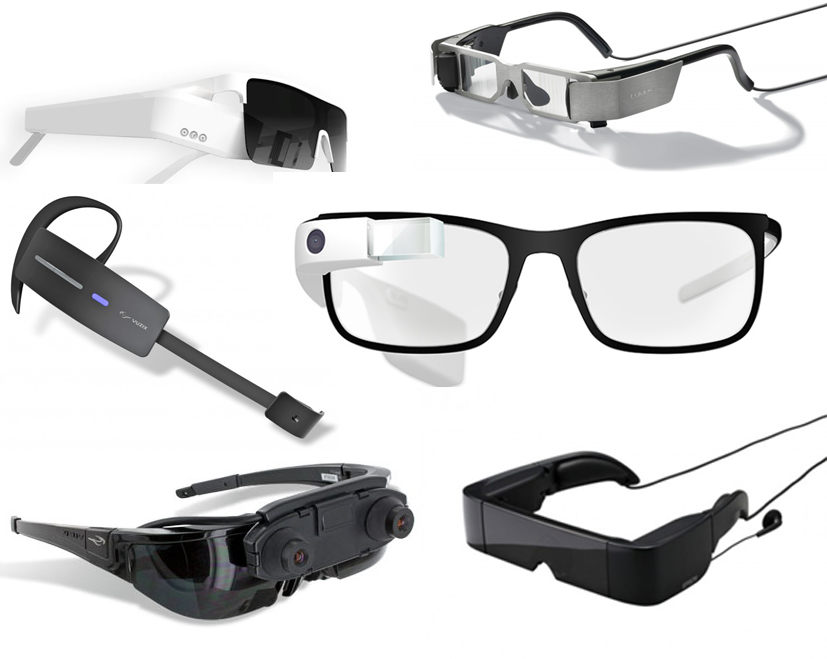
\includegraphics[width=0.8\textwidth]{chap1/ARGlasses}
  %\bicaption[fig:glasses]{增强现实设备}{增强现实设备}{Fig.}{Augmented Reality devices}
%\end{figure}

增强现实(Augmented Reality)是一种将虚拟场景融合进真实场景的技术,其中包括虚拟物体与现实的结合、即时互动以及三维的特性。
增强现实技术可以提供现实中无法获取的信息,用户通过附加的虚拟信息提升对现实场景的了解,增强现实技术在医疗、工业、娱乐与教育上都有广泛的应用前景。
Azuma等人在1997年和2001年\upcite{azuma1997survey,azuma2001recent}及Feng Zhou等人\upcite{FengZhou:2008:TAR:1605298.1605333}在2008年综述了增强现实所需的环境设置、追踪技术、交互技术、用户界面、显示技术及应用发展趋势。

而混合现实(Mixed Reality)则是介于虚拟场景和真实场景之间的一种形态,从图\ref{fig:mr}中看到Milgram\upcite{Milgram:2009:TDC:1643928.1643932}对混合现实,虚拟现实以及真实场景的渐变过程划分,混合现实包含了增强现实与虚拟现实。

\begin{figure}[!htp]
  \centering
  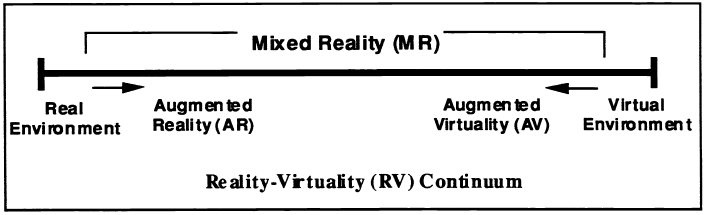
\includegraphics[width=0.95\textwidth]{chap1/Milgram_Continuum}
  \bicaption[fig:mr]{混合现实}{混合现实\upcite{milgram1995augmented}}{Fig.}{Mixed Reality\upcite{milgram1995augmented}}
\end{figure}

随着Google Glass\upcite{googleglass}的上市,智能眼镜成了2014年增强现实与混合现实领域最期待的设备之一。
%,从图\ref{fig:glasses}可见现在炙手可热的一批增强现实穿戴式设备。
眼镜最大的特征在于不需要用户手持进行操作,这一点诸如手机、平板或者更为累赘的台式机、笔记本是完全无法比拟的。
并且眼镜的视野十分宽阔,基本可以覆盖人眼的整个视野,虽然现在的手机越做越大,平板的普及性也很高,但是用户依然可以感受到这些智能设备的边界,而眼镜,就没有这样的局限性。
因而针对眼镜此类设备的研究及其与增强和混合现实应用的结合正是近些年来的研究热点。

针对不一样的设备,关于多点触控、手势、语音控制等多种交互通道的研究层出不穷。
一种类型的交互系统使用单一的通道进行交互,比如平板电脑上的多点触控,或者使用摄像头进行手势识别,再有些利用遥感等传感器进行不同指令的发送。
考虑到视觉通常会受到外界不相干信息干扰,语音控制也是非常直观的一种方式。
另一种类型的交互系统则综合多种通道协作进行交互,诸如利用压力传感,电流反馈等释放双眼、双手的交互方式。
%尽管手势交互因其直观在交互手段中占据了大部分应用,但多种交互手段的尝试对本文的研究是很有必要的。

除了交互手段对增强和混合现实应用有着举足轻重的影响以外,如何在不同的状态间切换、如何区分不同的状态,虽然是一个应用细节,却也极大地影响用户的使用体验。
同样的情形如果在桌面应用上,可能就是一个鼠标点击的区别,即便是最糟糕的情况也莫过于切换过于频繁,让用户很难继续之前的任务。

但在增强现实和混合现实的应用环境下,整个工作环境与输入空间都不是严格固定的,诸如最基本的拖拽还是单纯的移动都无法直接识别,需要通过其他的辅助或者设定才可以完成,因而对于不同交互手段如何在状态间切换也是一个研究热点。
目前状态切换存在着容易混淆\upcite{TrackingBased}、呈现不自然\upcite{Selection}及增加记忆负担\upcite{SideBySide}等问题,值得进一步研究。

与此同时,在对增强和混合现实应用的调研中发现,多数应用都涵盖模型的使用,而关于这点通常都以导入模型来处理。
导入模型虽然简单易行但受控于应用自身的数据库,而且用户无法根据自己的想法创建自定义的符合当前场景的模型。
针对三维建模这一应用场景,现下已经有很多相关的轻量级软件,可以通过简单的操作构建出复杂又美观的模型来。
但在增强和混合现实的应用条件下,哪些设计可以保留并提升,哪些需要舍弃则是另一个需要进一步探索的研究点。
因而需要对物体创建应用在不同的平台如桌面应用、手持移动设备和释放双手的穿戴设备做调研。

桌面应用普遍基于单击工具完成,如Google Sketch\upcite{sketchup}和TinkerCAD\upcite{tinkercad},对于工具的设计是一个很好的切入点。
而其他手持设备在基于单手操作的限定条件下对建模应用进行的设计就非常值得借鉴,比如指尖绘制,通过自制的标签笔进行绘制等,还有释放双手的场景中结合三维场景和平板同时进行模型设计的方法。
其中对于用户建模的难点主要集中在(1)如何克服用户自身不同的绘制水平,帮助用户改善自己的模型。(2)如何提供用户足够的自由度创建有自己特色的模型,不受限于应用的约束。

\section{研究目的}
\label{sec:xulun-mudi}
通过上述对当前背景的了解,本文的研究目的为自行制作一个混合现实眼镜、探索混合现实眼镜设备下直观的交互界面、研究便捷的交互方式及合适的三维建模方式。
为了更清楚地说明自制的混合现实眼镜上的交互界面与交互手段的设计,首先对相关设备、交互、建模和状态切换的研究现状进行详细阐述。
%本文旨在自制的混合现实眼镜上,研究适合此类随身携带的头戴式设备的交互系统,包括交互界面、交互方式及其他辅助方法,让用户使用该系统进行空间设计。
本文将总结研究现状的优点与不足,设计新的三维界面和操控方式,并在此基础上设计新的空间设计方法。
其中交互界面是新设计的一种三维界面,交互方式则是以手势输入为主,配合头部动作形成的多通道交互方式,以此来改善用户体验。
而空间设计方法则是针对三维建模的应用环境,辅助用户制作特制且优质的模型的三维建模方法。

\section{研究现状}
\label{sec:related-cur}
\subsection{光学透视与视频透视}
\label{sec:related-vst}
本文工作的整体实现需要依赖一个便捷的混合现实设备,眼镜。因而对于眼镜的种类及制作方式的调研为一切之基础。混合现实眼镜有两种制作方案,一种是光学透视式,用户透过眼镜镜片观察到真实世界,同时镜片上通过投影或其他方式实现虚拟场景的显示;另一种是视频透视式,镜片即显示器,用户通过镜片观察到已经将真实场景和虚拟场景融合的增强现实结果。FIGI\upcite{FIGI}在光学透视眼镜上无缝连接了数据手套操控和键鼠操控;Mime\upcite{MIME}则通过光学透视眼镜与TOF的结合进行了单手指尖识别。
与之相对,Ha等人\upcite{ha2006bare}通过视频透视眼镜对裸手进行分析与识别;
Looser等人\upcite{LookingGlass}通过视频透视眼镜对现场环境进行识别与操控。
光学透视眼镜在分辨率和视点无偏差上有着优势,但考虑到增强与混合现实应用中经常需要处理的真实物体与虚拟物体间的遮挡,和不同光线下光学透视眼镜受到的影响,本文最终决定通过一个视频透视眼镜来完成眼镜设备上的交互设计与菜单研究。

\subsection{增强现实与混合现实设备上的交互技术}
\label{sec:related-jiaohu}
为了决定在自制的混合现实眼镜下使用何种或者结合哪几类交互手段,本文对增强现实与混合现实设备上的交互方式做了深入的调研与分析。
最通俗常见的是手势交互,为了检测与追踪手部,一部分设备在制作上和交互方式上进行了专门的设计。
SideBySide\upcite{SideBySide}是一套手持相机投影仪套装,通过投影出来的不同影像进行交互,使用过程中使用者总是要被占用掉一只手是最大的不便。
Oakley和Park的工作\upcite{Pointing}通过对手持设备的甩动来进行交互,同样也有这个特点。
王晓春等人\upcite{王晓春2007基于笔交互的表格制作}以及H{\"u}rst等人的工作\upcite{TrackingBased}都设计了一个工具让用户手持进行交互。
王晓春等人\upcite{王晓春2007基于笔交互的表格制作}设计了基于笔的交互,通过对草图的字线分离实现了一种灵活的表格制作方法,在徒手绘制物体方面值得借鉴。
H{\"u}rst等人\upcite{TrackingBased}在一支普通的笔两端绑上了两个图案(pattern)便于识别,进行物体建模,这样的工具在识别和使用上都很有优势,然而在交互直观性上略有欠缺。
同样利用特殊标记(marker)的还有Chun等人的工作\upcite{Chun:2013:RHI:2449396.2449435},通过设计多个单手手势通过移动设备的摄像头对虚拟物体进行位置、大小以及透明度的调整。
而uTrack\upcite{uTrack}则是通过在拇指和其他手指上佩戴磁力感应器,分析其位置和倾斜角来设计手势。
这一类佩戴在手指上的设备解决了手持类设备的问题,释放了双手,但此类设备最大的问题在于,若是使用过程中设备佩戴的位置或角度产生了变化,则会对之后的分析都产生影响,导致不可估的后果。
Datcu和Lukosch\upcite{datcu2013free}设计了一套交互手段,用户穿上指定的衣服用来降低手势检测的复杂性,佩戴上视频透视眼镜后,可以通过特定的手势进行调用菜单和浏览的操作。
相比于手上佩戴复杂的设备,穿着指定的衣服虽然普遍性低,但保持了手部的轻便。
FIGI,Witt等人和王修晖等人的工作\upcite{FIGI,Maintenance,王修晖2007面向多投影显示墙的手势交互系统设计与实现}都借助了数据手套,
FIGI\upcite{FIGI}利用两手间的向量对物体进行操控;
Witt等人\upcite{Maintenance}利用手套得到手部的旋转信息来进行交互;
王修晖等人\upcite{王修晖2007面向多投影显示墙的手势交互系统设计与实现}测量手指的关节动作,结合手掌弯曲的程度设计了三种手势进行交互。
虽然数据手套没有占用使用者的手,但其不适感还是降低了用户体验。

另一部分设备则通过特定的输入设备对裸手进行捕捉,从而来识别手势与追踪,这一类设计的最大优势就是还原了手势交互的自然特性,本文工作也将借鉴此优点。
Tamaki等人\upcite{BrainyHand}设计了两种交互方式,简单版本通过相机捕捉三种手势进行指令的发送,这是一组单手交互;
投影版本则是投影菜单列表在一只手上,另一只手进行拣选操作,这是一组双手交互。
Tamaki等人展现了一组轻便的手势交互,但设计的单手手势和发出的指令没有对应联系,需要使用者额外的记忆,
而双手交互中,投影的菜单列表就像投影仪投影在墙壁上的观感一样,没有充分利用世界的三维特性。
孙超等人\upcite{孙超2011增强现实环境下的人手自然交互}通过区域检测跟踪一系列算法获取人手的三维结构,然后以指尖轨迹、指向拾取和手掌托取三种手势进行交互。
通过这三种手势实现3D笔画、射线拾取和手掌托物,但在对物体的基本操控上,这些设计覆盖得还不够完整。
以Kinect为代表的深度相机在这类交互中发挥了重要作用。
虽然其获得的深度数据噪点很多,但深度图像提供的深度信息对分割不同的物体有很大帮助\upcite{oikonomidis2011efficient}。
然而深度相机对于用户来说比较笨重且耗电严重,因此在Mime\upcite{MIME}中采用了三个TOF作为识别设备,通过分析处理三个TOF设备的信号检测用户单手手指的指尖来进行基于点的交互。当背景变幻的时候由于TOF设备只对距离敏感,因而不会造成信号的波动,达到了极高的稳定性,不过单手交互是现存的缺陷之一。

手势交互之外,通过语音,触觉,头部动作等的交互方式也是相关领域正在研究的交互手段。
早在2003年Brewster等人\upcite{MultiModal}就提出了解放人眼的交互方式,大部分用户极大地依赖人眼获取信息,使得人眼被许多信息占据,因而阻塞了获取信息的速度。
这里使用语音作为输出,呈雷达状披萨型菜单,通过旋转头部来进行菜单选取。Brewster等人还提出了一种皮带型菜单,用户不需要观察手指触碰的位置,而通过语音的输出来判断手所在的位置进行进一步的选择,就如同盲打键盘一样,盲打依靠的是用户对键盘的记忆,而这里的设计依靠的是语音的提示。
然而当周围环境喧闹的时候,语音的提示就无法起到效果,Azenkot等人\upcite{DigiTaps}设计了一种用一至三根手指表示所有数字的方法来减少对声音的依赖,通过三根以内的手指进行组合完成0-9十个数字的编码,虽然实现了盲打,既不依赖视觉也不依赖听觉,但精确性降低了。

还有一些新颖的交互方式如通过获取神经数据用脸部表情进行操控\upcite{Mimetic},主要通过颏肌、额肌和唇肌的运动来输出指令,通过压电膜(piezo film)来检测肌肉的运动,颏肌额肌的变化表示鼠标的上下移动,唇肌的运动表示选择与放弃选择;
还有一种提议将指甲变成一个触摸屏\upcite{chan2013fingerpad},在指甲上进行触控,这个设计的亮点就在于许多投影式设备和屏幕越来越大的手机已经丧失了对个人信息的私密性,而指甲上的触控则关注了个人信息的隐私性。
同样文献\cite{Eye-q}考虑到提供私密的信息,考虑到用户在不同的工作量情况下,对可视化信息的关注度是不同的,不仅如此,提供的提示信息并不能影响到用户当前的行为,故而其提示的方式也会调整成不过于引人注目的方式。
文献\cite{vidal2013pursuits}则是直接使用眼睛的移动路径来作为交互输入,不同的路径形状及顺时针逆时针方向都能导致不同的命令。

综上所述,增强现实与混合现实设备上的交互技术覆盖面非常广泛,而何种交互方式对用户而言最容易使用且效果最好则是该类设备上最值得探讨的问题。本文将以手势交互为主,配合其他肢体语言如头部动作、以空间设计为应用场景,对包括三维建模、三维操控等功能进行进一步的研究,来探索眼镜这类新型设备对空间设计类应用的辅助。

\subsection{增强现实与混合现实应用中的状态切换}
\label{sec:related-zhuangtai}
状态切换作为增强现实应用中的一个细节,在技术领域通常被人忽视,但作为一个追求用户体验的系统,这是一项必不可少的需要留意的设计。
如前文所提,自然交互和传统桌面应用的键鼠交互很大的不同在于状态与状态间没有明显的差异。
比如区别点击拖拽的动作和单纯移动的动作。针对这一细节有些前人工作采用了按钮,简单明朗但属于额外设计。
如Looser等人\upcite{LookingGlass}在一个手持的追踪球上增加了几个按钮作为操控。
类似的,Willis等人在\upcite{SideBySide}一个手持相机投影组的项目中增加了数个按钮设计了一套面向儿童的交互技术。
除此之外Zhou等人\upcite{Selection}用色环和标记作为辅助在书籍上进行多种选择方式的评估。比较遮盖标记做选择和露出标记做选择两种方式。
然而该系统使用色环和许多标记呈现出非常不自然的交互景象。
在Lee等人的工作\upcite{lee2010contact}中设计了一个由标记组成的立方体,通过该立方体进行菜单的显示,旋转该立方体则可以出发选中命令,非常新颖。
而Oakley\upcite{Pointing}针对点击这一特定操作设计了三种方法进行评估。该工作将白色长方体状的传感器分别放在手背,手腕和手心上进行用户体验与操作效果的实验。
同样是使用标记,H{\"u}rst等人\upcite{TrackingBased}将两个标记固定在用户的食指上,使食指成为一个增强现实的交互媒介,当用户遮住其中一个或两个标记时就会向系统发出对应模式的指令。
遗憾的是因为交互过程中还有许多其他需要留意的部分导致用户经常忘记在对应的时刻遮住对应的标记来发送模式指令,因而造成无操作。也由此可见不同的状态间的切换方法必须明显且易操作。
更有一部分工作设计的系统没有明显的状态切换,如Mime和Ha与Woo的工作,其涉及的应用类似水果忍者或者写便签\upcite{MIME,ha2006bare}。
本文一共设计了三种手势并且设计了手势之间的逻辑关系来避免混乱的状态切换,第\ref{chap:interaction}章将详细描述。

\subsection{基于手的交互}
\label{sec:related-shou}
在对前人工作的研究中,手势交互是数量最大的一类,而本文也将以设计手势交互为主,考虑到不同的设备对手有不同的约束,手持设备如手机、平板或其他特殊设计将占用一只手,而其他穿戴式设备如眼镜等释放了双手,因此本文将针对单手交互和双手交互分别作背景调研。

单手交互如H{\"u}rst等人\upcite{TrackingBased},其设计了一个手机平台上的模型创建应用。
用户在摄像头前方进行操控,通过手机屏幕看到建模的结果。然而在实验结束后用户反馈一只手一直保持举着手机的姿势有些劳累,而且用户通过手机屏幕观察到的场景与直接肉眼观察到的现场存在着视觉偏差也降低了用户体验。并且手部与眼睛之间的坐标转换也是一个问题。
Lee等人\upcite{Lee:2009:FIM:1643928.1643961}同样也是在手持设备上进行交互设计,针对手持设备的摇晃(shaky)状态,特别设计了Freeze-Set-Go的交互方法,先将场景固定,然后进行交互,但对于习惯自由交互的用户来说额外增加的一个步骤就显得有些累赘了。
而HIT Lab\upcite{Bai:2013:FIH:2543651.2543667}在手持设备上安装了深度相机,通过色彩和深度信息提取手的骨骼,然后将基于手势的交互方式与键盘和触摸屏进行比较,通过对虚拟物体的平移、旋转和缩放得出手势交互更为直观的结论。
文献\cite{MIME}提供了一个单手识别与交互的头戴式显示设备。作为一个头戴式设备释放了双手,且能在嘈杂纷乱的背景保持指尖检测的准确度,但单手交互限制了他的多样性。
因而从人体工程学的角度出发,本文将设计一个释放双手的设备且支持双手交互的系统,让用户可以舒适实用且有更多的手势选择。本文计划制作的混合现实眼镜不仅解决了这些缺陷同时避开了手眼坐标不一致的问题。

双手交互如Tamaki等人的Brainy hand\upcite{BrainyHand},其为一个轻便的穿戴式设备方便用户每日穿戴。
该系统通过投影仪将菜单投影到一只手上,另一只手对菜单列表进行拣选,这里Tamaki等人将不同的职责分配给了不同的手,右手作为一个操作工具而左手则是操作区域。
这一点设计经验证对用户使用来说非常自然而且对本文的设计也有很大启迪。

另外,HIT Lab\upcite{Bai:2014:GIH:2669062.2669073}对裸手的三维手势与手持设备下的单手手势进行了性能与用户体验评估。
通过三维空间内的平移旋转缩放验证三维手势交互的可行性,虽然长时间持有手机、平板等移动设备让用户觉得不适,但自由的三维手势比触摸板上的手势更受用户亲睐,更具有交互的研究前景。

因而本文采用自由的三维手势,且着重关注了双手交互设计的原则。
对此Hinckley\upcite{hinckley1998two}曾讨论过三项重要原则:
\begin{enumerate}
	\item 由右及左 \hfill \\		由用户的惯用手负责更细节精确的工作而由非惯用手承担控制方向或位置的粗颗粒度工作。
	\item 移动规模的不对称 \hfill \\		不同的手对于移动和工作空间的规模设计是不一样的,比如左右手移动相同的距离而造成工作环境下的移动距离应该不一样。
	\item 左手先行 \hfill \\	
	左手用以启动整个操作流程。
\end{enumerate}

而后Hinckley以一个洋娃娃模型的观察作为具体介绍实例。
用户通过手持一个洋娃娃作为控制一个模型的代理,用非惯用手通过该代理控制目标物的方向和大小,用惯用手握住一个切割平面来告诉系统现在想观察哪个平面。
在该应用环境下双手的交互设计配合默契。
然而,虽然手持一个代理增加了不少操控的真实感,但也减弱了本文系统的可移植性且增加了配置的复杂度。
除此之外Cutler等人的工作\upcite{cutler1997two}中也提及了双手交互的不对称性。
本文将取之所长设计一套轻量级的双手交互系统,结合本文涉及的交互方式与应用场景重新评估三项重要原则的可行性,让用户可以自在地设计自定义模型。

\subsection{物体创建}
\label{sec:related-create}
建模软件在桌面应用中屡见不鲜,且慢慢地从专业设计人员使用的复杂应用转向轻量级。
如Google Sketchup和TinkerCAD,其中TinkerCAD提供了一系列预定义物体组件供用户选择\upcite{sketchup,tinkercad}。
这些组件可以添加到场景中或从场景中挖去相应体素的凹洞,任意物体都能旋转放缩,整个应用非常简单易学并且有强大的物体组件库。

相对于预定义组件,另一种建模方式就是绘制草图。
Bergig等人\upcite{bergig2009place}采用的方式是就是先进行草图绘制,然后通过数据库识别出物体种类将二维草图转为三维物体。
整个过程包括对草图图像的理解和物体重建。
其更接近于一个识别系统而非建模系统。
但如果系统数据库中包含了足够多用户会绘制的物体,其能达到非常完美的匹配效果。
Redondo等人\upcite{Redondo:2014:EQA:2669711.2669938}针对数字涂鸦(digital sketch)在教育中的用途展开了评估。
结果表明增强现实的显示方法对数字涂鸦的效果有很大帮助。

还有一类类似的方法,称之为自动模型创建,从二维图形中提取为三维模型。
Zollmann等人\upcite{Zollmann:2012:DDM:2407336.2407347}结合通过形状识别、数据库提供的语义信息与视觉提示(cue),通过已有的轮廓图案、地理数据库中的点与线条和深度信息,提出了一种图像分割算法判断深度与遮挡信息,最终基于图像进行建模。
Clifford等人\upcite{Clifford:2011:UAR:2000756.2000774}则在房屋建设的天气下,通过房屋的建筑图进行分析,将点的信息从不同的特征中提取出来,将线的候选者延伸为墙壁,组成房屋的三维模型,特别该文还使用了多人协作进行模型显示,促进了最后的展示效果。
同样利用语义信息的还有Chen等人的工作\upcite{Chen:2014:ASM:2661229.2661239},通过深度相机捕获粗糙的输入图像然后利用数据库中大量的室内场景信息进行语义分析,进一步判断捕获场景中的物体的上下文,然后对物体进行建模。
而在本文中,我们更倾向于使用自由绘制的方法,使用户可以创建任何他们所想的独一无二的模型。
除此之外,Schkolne\upcite{schkolne2002drawing}在一个半沉浸式环境中构建了一个面向艺术家的绘制系统,通过对绘制结果的二次处理呈现了非常惊人的艺术效果,然而考虑到本文系统更多针对普通人群,因而本文系统会提供更多帮助面向原先并不擅长建模的人们。

在从零开始进行的模型创建之外,还有关于对真实世界的物体进行克隆与编辑的工作。
ClonAR是Csongei等人\upcite{Csongei:2012:CRR:2473501.2474179}通过Kinect Fusion进行扫描,然后在增强现实的环境下用标记数据域(Signed Distance Field)对物体进行二次编辑的工作。
该工作的特点在于快速扫描与二次修改。
其中Kinect Fusion是一个通过移动的Kinect对场景进行捕获,然后通过深度数据快速三维重建的系统\upcite{Izadi:2011:KRD:2037826.2037857,Izadi:2011:KRR:2047196.2047270,kinectieee},
有其他重建类工作基于Kinect Fusion研发而成\upcite{Shao:2012:IAS:2366145.2366155,Zhou:2013:DSR:2461912.2461919},
考虑到本文对输入设备的考虑,Kinect Fusion依赖Kinect,而Kinect对于眼镜类混合现实设备稍显笨重,故暂时不在考虑之中。

H{\"u}rst等人\upcite{TrackingBased}则是在移动增强现实环境下提出了虚拟网格这一辅助工具帮助用户进行创建物体。
虚拟网格与用户创建的物体表面对齐,用户可以将网格附着在不同表面上然后在不同的方向上继续创作,增加模型的多样性。这一想法启迪了我们,我们分析到该虚拟网格受限于物体的表面坐标轴,也因此限定了用户一定的交互,于是本文提出自由虚拟网格平面达到更高的操控度,也更适合混合现实眼镜下的空间建模。

\section{本文工作成果与创新点}
本文的主要成果体现于混合现实眼镜的制作、混合现实眼镜下的人机交互设计、双手交互的设计原则以及对本文所设计系统的评估。
\begin{enumerate}
\item 混合现实眼镜的制作\hfill\\
首先设计并制作硬件,本文的研究工作全部建立在该眼镜的制作上,而其配置也经历了从早期的笨重版本到混合现实眼镜轻量级的演化。
\item 三维操控及辅助方法的设计\hfill\\
同样为了配合三维的应用空间,这里针对单手和双手分别设计了不同的交互手段,
单手的交互更接近于触屏操控,只不过屏幕为空中的任意平面;
双手的交互无需选择命令,因而可以同时进行多项操控。
在完成了混合现实眼镜下的的可行性分析后,针对实验者的表现情况和反馈设计了更多辅助用户交互的方法,增加了顶置提示板、骨骼小球和头部约束。
\item 双手交互设计原则的更新\hfill\\
根据\ref{sec:related-shou}节,Hinckley\upcite{hinckley1998two}曾讨论过的三项双手交互重要原则结合现在的应用环境重新设计了本文系统的双手交互设计原则。
分别是由右及左,对称的工作规模和右手先行。
之后对于用户进行空间设计的具体操作均考虑了这三个基本原则。
\item 可行性与易用性评估\hfill\\
本文评估了所设计的三维菜单与布局在混合现实眼镜下的可行性,及结合头部约束、顶置提示板、骨骼小球的单手及双手操控交互的易用性。
\end{enumerate}

本文的创新点主要由三维菜单的设计、自由虚拟网格平面的设计和职责分离的双手概念组成:
\begin{enumerate}
\item 三维菜单\hfill\\
基于增强现实所处的三维操作空间设计独有的三维交互界面,本文工作借鉴了画家画画的寓意将一款菜单设计在手掌之中,而形状和人手本身,调色盘接近,视为原型。同时考虑到不同的需求设计了三种布局,分别是手掌召唤式菜单,目标跟踪式菜单和屏幕固定式菜单。并在之后的实验环节进行了详细的评估。并分析了三种布局的偏好。
\item 自由虚拟网格平面的设计\hfill\\
为了帮助用户既能创建具有自己特色的独一无二的模型,又能尽量消除普通人并不擅长建模的缺点,本文所设计的系统基于H{\"u}rst等人\upcite{TrackingBased}的虚拟网格平面想法作了进一步深化,加强了其可操作度,针对朝向和大小进行了特别的操控设计。
\item 双手职责分离的设计\hfill\\
出于无缝状态切换与无间断建模的目的考虑,本文工作将左右手的职责分开,分别为绘制之手和操控之手,而在建模途中两只手可以同时操作,达到在工具切换过程中无需中断建模过程的效果。
\end{enumerate}

\section{论文组织结构}
本章首先介绍了本文的研究背景,通过对增强现实及混合现实的设备、技术与应用了解,归纳本文的研究目的,然后详细调研了相关背景的现状,最后总结本文工作的成果与创新点。

第\ref{chap:system}章先介绍本文工作采用的研究方法,而后是对本文所设计系统的概览。
概览包括系统的功能分布、大致流程及使用的自制眼镜制作历史与方法。
其中针对系统划分成多个模块,便于更好的设计与阐述。
对自行制作的眼镜从其几个版本的变化来论述用户对此类设备的要求及其发展趋势。

第\ref{chap:3DUI}章是具体设计的第一个部分,针对混合现实眼镜的三维界面设计。本文将从设计的出发点开始阐述整个界面的设计,并且基于对布局可能造成用户体验不同的假设,设计了多种布局与实验。

第\ref{chap:interaction}章是具体设计的第二个部分,详细介绍本文系统所采用的空间交互设计,主要以手势设计为主,配合其他的通道和提示,辅助用户可以更好地与系统进行交互。

第\ref{chap:3DModel}章是具体设计的第三个部分,对三维建模进行详尽设计并展示其应用场景。
通过对前人在物体创建方面的研究,该章会介绍本文特有的双手建模方法,然后阐述三维建模应用场景研究与结果。

第\ref{chap:exp}章是针对本文所做的设计与应用进行的用户实验,通过不同背景的参与者的体验来评估本文所设计与实现的交互界面与手段的可行性与易用性。

第\ref{chap:conclusion}章,最后一章将对本文的工作进行总结与展望。
%%==================================================
%% chapter02.tex for SJTU Master Thesis
%% based on CASthesis
%% modified by wei.jianwen@gmail.com
%% Encoding: UTF-8
%%==================================================

\chapter{研究方法与系统概览}
\label{chap:system}
继第\ref{chap:what}章阐述了本文的研究背景与目的后,本章将进一步介绍本文研究所采用的方法。其中,视频透视技术用于制作混合现实眼镜;
而融合本文所设计的系统多设备间的手势识别技术则用于结合本文所设计的系统所涉及的多种设备输入,使之识别更稳定的手势;最后,针对帮助用户更好地建模而采用沿法向拉伸的自由虚拟网格平面。
此处为基本的技术提要,在第\ref{chap:interaction}章对手势识别有更详细的补充,第\ref{chap:3DModel}章对自由虚拟网格平面的设计有更多的说明。
然后本章将系统划分为多个模块一一介绍,先基本了解本文系统的组成部分,以便进一步深入细节。
\section{研究方法}

\subsection{视频透视技术}
考虑到增强与混合现实应用中经常需要处理的真实物体与虚拟物体间的遮挡,和不同光线下光学透视眼镜受到的影响,本文决定制作一个视频透视\upcite{rolland2000optical}眼镜来完成本文的研究工作。
视频透视技术通过相机拍摄真实场景,利用数字图像处理的方式从图像中获得信息,让佩戴者通过观察数字图像感知真实场景,其中涉及双目相机的标定与图像校正来制作视频透视眼镜,将实际见到的场景经过变化后作为眼镜的输入。
通过得到两个相机的内参与所拍摄的图像进行双目标定与校正,计算其相同点在不同相机中的位置,得到视差,通过视差计算三维坐标数据,因而得到两个相机的外参,而后对两个相机获取到的图片进行校正。

\subsection{融合视觉和LeapMotion的手势识别技术}
考虑到本文工作将采用双目相机和Leap Motion作为输入系统,本文工作决定融合双目相机的输入,与Leap Motion\upcite{motion2012leap}结合,获取更稳定的手势信息。
本文所设计的系统利用OpenCV\upcite{opencv}双目标定对双目相机进行标定,再与LeapMotion标定,从而得到当前场景手的关键点的坐标和色彩信息。
然后对每个设计的手势进行样本采集,分别训练每个手势。
结合LeapMotion得到的手的关键节点信息,当手的节点坐标与手的形状同时满足所设计的手势要求,则识别成功。
为了增加手势识别的稳定性,每个手势的识别会考虑邻近帧的情况,将邻近帧中被成功识别的手势作为参数之一。
考虑到用户在操控时自制的混合现实眼镜会有轻微地抖动,系统将比对邻近帧判断用户是否正在进行三维建模与操控,此处基于所有操作都不会需要大幅度移动的假设,如果正在进行三维操控,则增大邻近帧参数数值保证手势识别的稳定性,如果用户正在浏览场景,则不对手势进行识别。

\subsection{法向拉伸的自由虚拟网格平面技术}
自由虚拟网格平面是本文工作针对混合现实眼镜下的三维建模所设计的一个辅助方法,
沿法向拉伸是自由虚拟网格平面的特性。
自由虚拟网格平面将支持用户在建模期间以一个虚拟网格作为参照物,默认时虚拟网格以水平方向呈现,所有物体都在水平方向上延伸,最小单位为一个虚拟单元格。
用户可以通过先建模物体的一个面,然后执行法向拉伸的操作使之成为一个三维物体。
拉伸过程中调整虚拟网格的朝向,进一步调整物体使物体可以往垂直,斜切等其他方向延伸,而后用户可以在该网格上进行不同朝向的建模,构建更丰富的模型。
拉伸过程中同样可以调整虚拟网格的大小,创建不同形态的模型。

\begin{figure}[!htp]
  \centering
  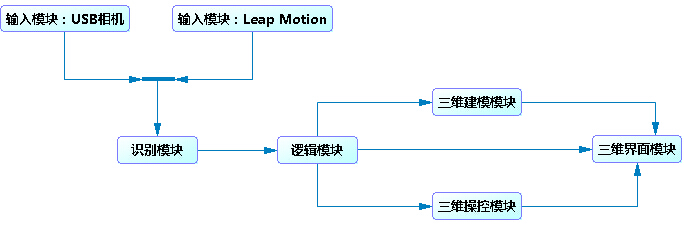
\includegraphics[width=0.8\textwidth]{chap2/system}
  \bicaption[fig:process]{系统概览图}{系统概览图}{Fig.}{system diagram}
\end{figure}

\section{系统介绍}
\subsection{系统概览}
本文系统着重研究混合现实眼镜下的交互界面、交互手段及空间设计应用中的具体设计,图\ref{fig:process}所示本文系统主要分为这几个模块:
输入模块、多通道识别模块、三维界面模块、逻辑模块、三维操控模块与建模模块。

%\begin{figure}[!htpb]
  %\centering
  %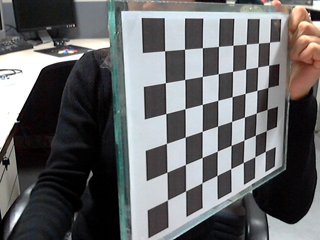
\includegraphics[width=0.24\textwidth]{chap2/camera_0_cap_1}
  %\hspace{1cm}
  %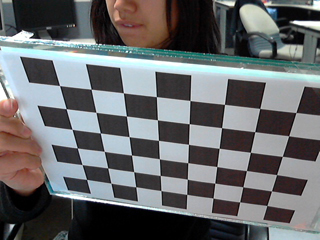
\includegraphics[width=0.24\textwidth]{chap2/camera_0_cap_2}
  %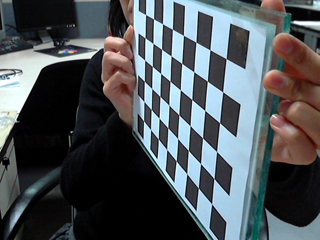
\includegraphics[width=0.24\textwidth]{chap2/camera_0_cap_12}
  %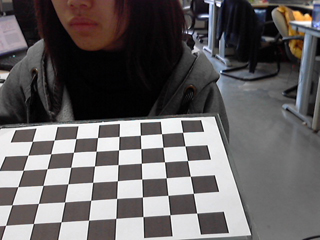
\includegraphics[width=0.24\textwidth]{chap2/camera_0_capture_1}
  %\bicaption[fig:chess]{棋盘格标定}{棋盘格标定}{Fig.}{Chessboard calibration}
%\end{figure}

\begin{figure}[!htpb]
	\centering
	\subfigure{\label{fig:chessboard:1}}\addtocounter{subfigure}{-2}
	\subfigure[Turn right]{\subfigure[向右偏转]
		{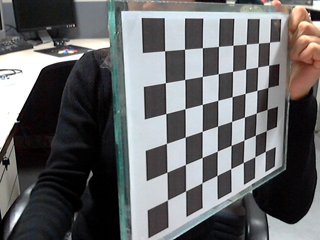
\includegraphics[width=0.22\textwidth]{chap2/camera_0_cap_1}}}		
	\subfigure{\label{fig:chessboard:2}}\addtocounter{subfigure}{-2}
	\subfigure[Turn down]{\subfigure[向下偏转]
		{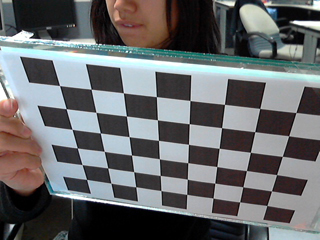
\includegraphics[width=0.22\textwidth]{chap2/camera_0_cap_2}}}		
	\subfigure{\label{fig:chessboard:3}}\addtocounter{subfigure}{-2}
	\subfigure[Turn left]{\subfigure[向左偏转]
		{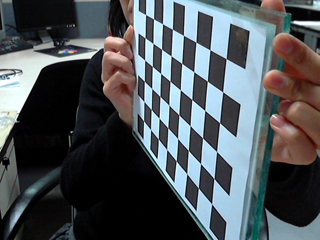
\includegraphics[width=0.22\textwidth]{chap2/camera_0_cap_12}}}	
	\subfigure{\label{fig:chessboard:4}}\addtocounter{subfigure}{-2}
	\subfigure[Turn up]{\subfigure[向上偏转]
		{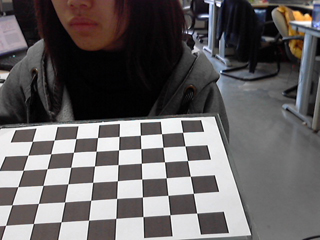
\includegraphics[width=0.22\textwidth]{chap2/camera_0_capture_1}}}		
	\bicaption[fig:chess]{棋盘格标定}{棋盘格标定}{Fig.}{Chessboard calibration}
	%\bicaption[总标签名]{}{中文总标题}{Fig.$\!$}{The total caption}
	\vspace{-1em}
\end{figure}

\subsection{输入与识别模块}
\label{sec:input}
	
本文系统在设计过程中涉及多种输入方式,本模块负责所有输入的标定。本文所设计的系统使用自制的混合现实眼镜ARGlasses作为系统输入,ARGlasses在演变过程中由不同硬件设备组成,输入部分有USB Camera, Leap Motion及改装过的广角USB Camera。 
为了模拟双目视觉的效果,系统之初采用两个横置USB Camera,
如图\ref{fig:chess}所示通过棋盘格进行独立标定,获得所需内参,图\ref{fig:chess}(a)、\ref{fig:chess}(b)、\ref{fig:chess}(c)和\ref{fig:chess}(d)分别是上下左右四个方向尽力偏转标定的演示,而后再进行双目标定。
图\ref{fig:stereoCalibration}显示通过双目标定后对原图像进行变换,变换前可从图\ref{fig:stereoCalibration}(a)中观察到左右二图的不匹配,而后左右眼图像(图\ref{fig:stereoCalibration}(c)})对齐效果更佳,可从背景的一些水平纹理中看到。
\begin{figure}[!htpb]
  \centering  
  \subfigure{\label{fig:stereoCalibration:before}}\addtocounter{subfigure}{-2}
	\subfigure[Left image before calibration]{\subfigure[标定前的左图]
		{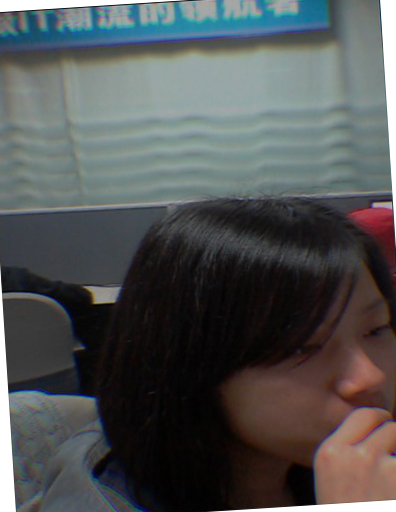
\includegraphics[width=0.225\textwidth]{chap2/beforeCalibration}}}		
	\subfigure{\label{fig:stereoCalibration:beforer}}\addtocounter{subfigure}{-2}
	\subfigure[Right image before calibration]{\subfigure[标定前的右图]
		{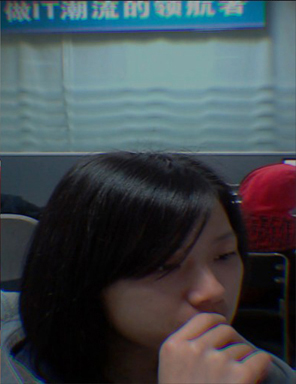
\includegraphics[width=0.225\textwidth]{chap2/afterCalibrationR}}}		
	\subfigure{\label{fig:chessboard:3}}\addtocounter{subfigure}{-2}
	\subfigure[Image after calibration]{\subfigure[标定后的图]
		{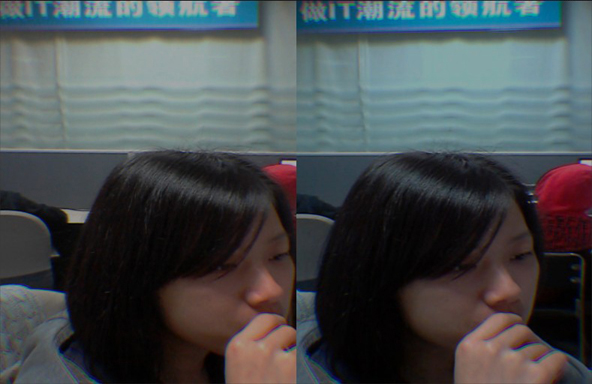
\includegraphics[width=0.45\textwidth]{chap2/afterCalibration}}}	
  \bicaption[fig:stereoCalibration]{双目标定}{双目标定}{Fig.}{stereo calibration}
\end{figure}
然后Leap Motion的采用是为了获得更稳定细致的手势信息,早期Leap Motion只提供具体的手部骨骼信息,为了将相机输入信息与Leap Motion的手部骨骼信息融合,系统自行设计了一套标定方法,系统通过在相同的位置呈现手势与棋盘格,获得多组对应数据进行点集映射得到粗略标定结果。
为了扩大捕捉到的场景视角,系统给相机增加了广角镜头,因此在输入处理过程中先对广角镜头捕获到的画面进行反扭曲处理,而后对反扭曲的结果进行棋盘格标定等操作,其效果可由图\ref{fig:WideLensUndist}可见。
棋盘格在图
\ref{fig:WideLensUndist}(a)中交叉线微微弯曲,而在图\ref{fig:WideLensUndist}(b)中反扭曲为直线,可见效果。

\begin{figure}[!htpb]
  \centering
  \subfigure{\label{fig:WideLensUndist:before}}\addtocounter{subfigure}{-2}
	\subfigure[Image before wide lens undistortion]{\subfigure[广角镜头反扭曲前的图]
		{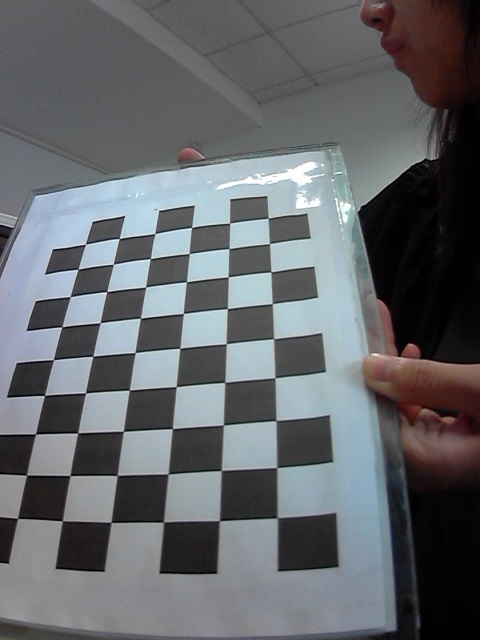
\includegraphics[width=0.3\textwidth]{chap2/camera_1_capture_6}}}		
	\subfigure{\label{fig:WideLensUndist:after}}\addtocounter{subfigure}{-2}
	\subfigure[Image after wide lens undistortion]{\subfigure[广角镜头反扭曲后的图]
		{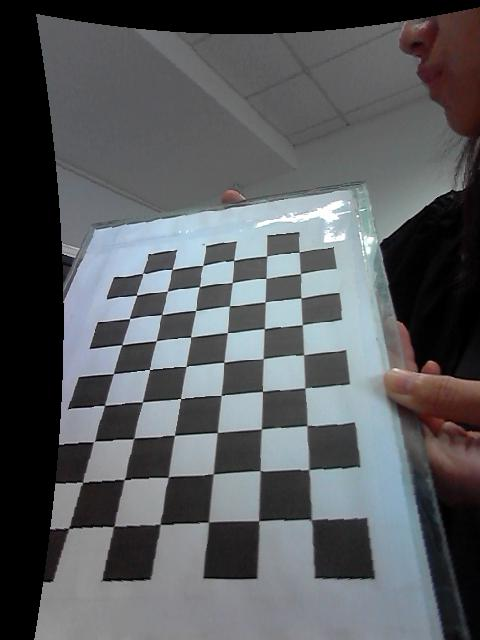
\includegraphics[width=0.3\textwidth]{chap2/undistcamera_1_capture_6}}}
  \bicaption[fig:WideLensUndist]{广角镜头反扭曲前后对比图}{广角镜头反扭曲前后对比图}{Fig.}{Undistortion of USB camera with wide lens}
\end{figure}

在研究的过程中,Leap Motion提供图像接口,可以获取拍摄所得源图像,于是系统结合Leap Motion所获取的源图像与相机图像进行匹配。
通过Leap Motion得到的原图进行反扭曲处理,由图\ref{fig:LeapMotionUndist}可见前后对比,棋盘格在图
\ref{fig:LeapMotionUndist}(a)中向右偏转,图\ref{fig:LeapMotionUndist}(b)中正面向前,图\ref{fig:LeapMotionUndist}(c)中向右偏转,然后将其作为混合现实眼镜的背景。
本模块最终输出标定过后的图像或手势信息,供识别模块进一步处理。
虽然输入模块相当重要,但并非本文重点所以之后并不再赘述。

\begin{figure}[!htpb]
  \centering
  \subfigure{\label{fig:LeapMotionUndist:left}}\addtocounter{subfigure}{-2}
	\subfigure[Turn right]{\subfigure[向右转]
		{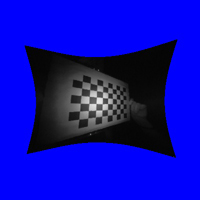
\includegraphics[width=0.3\textwidth]{chap2/undistort_399}}}		
	\subfigure{\label{fig:LeapMotionUndist:face}}\addtocounter{subfigure}{-2}
	\subfigure[Face to face]{\subfigure[正面]
		{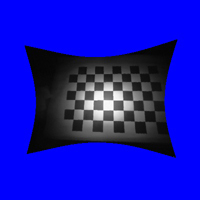
\includegraphics[width=0.3\textwidth]{chap2/undistort_299}}}		
	\subfigure{\label{fig:LeapMotionUndist:right}}\addtocounter{subfigure}{-2}
	\subfigure[Turn left]{\subfigure[向左转]
		{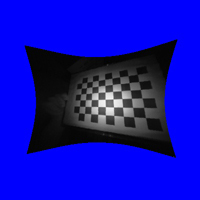
\includegraphics[width=0.3\textwidth]{chap2/undistort_219}}}
  \bicaption[fig:LeapMotionUndist]{Leap Motion反扭曲图}{Leap Motion反扭曲图}{Fig.}{Undistortion of Leap Motion images}
\end{figure}

识别模块主要有相机识别手势,Leap Motion识别手势,Oculus VR\upcite{Oculus}识别头部动作构成。
相机识别手势有以下几个步骤,首先获取原彩色图进行肤色提取,考虑到色彩空间在不同光线下并不稳定,所以这里设定了较广的肤色阈值,而后对超过手型大小阈值的肤色区域进行手型识别,根据形状判断是否含有手指,含有合法手指的区域便认定为是手型。标准的手型提取便是如此,之后根据手势的设计会有更细致的修改。
Leap Motion识别手势比较便捷,该设备官方提供手部骨架,可以直接分析其动作。
Oculus VR内置传感器,可以获得当前设备的角度,因而可以分析头部的动作信息,判断是否上仰。

\subsection{三维界面模块}
\label{sec:interface}
三维界面模块维护文所设计的系统界面,本文系统为混合现实眼镜设计了独有的三维界面,用来更好地配合用户的操作进行显示与交互。
三维界面由调色盘菜单和其他辅助信息组成,调色盘菜单地位等同桌面应用下的WIMP系列\upcite{Behr:2008:CND:1401132.1401164},负责让用户更直观地选择想要的命令。
其他辅助信息包括选中的立体包围盒,顶置提示板,骨骼小球都是本文所设计的系统运行中帮助用户更好地体验混合现实眼镜的可选配置,将在第\ref{chap:exp}章详细描述并评估。

\subsection{逻辑与操控模块}
\label{sec:logic}
逻辑模块负责连接识别结果与具体操作。结合识别到的手势,当前的环境,判断手势想表达的含义,比如在菜单出现时单手手指表示选择,而在物体被选中时表示单手操控。
据此调整三维界面上的显示,包括在顶置布告栏上更新状态,更改被选中的菜单样式进行提醒等。
逻辑模块还将输出具体指令下的操作参数,如旋转操作的轴参数与角度参数,传递给三维操控模块。

三维操控模块负责基本的平移旋转和缩放操控,通过输入的参数判断是哪种操控类型,然后根据参数进行实施操控,包括单手旋转和双手旋转时不一样的操控方式,也在该模块的处理之中。

\subsection{建模模块}
\label{sec:model}
建模模块针对三维建模用例,负责将用户的一系列建模指令转换成顶点。根据本文系统设计的自由虚拟网格平面,用户的输入全部转化为控制点,根据控制点该模块将绘制网格形成三维模型。
由于控制点的顺序随用户自定,所以该模块首先根据所有的控制点进行最优凸多面性估测用户绘制的形状,然后将不同层之间的控制点连接成三角面片。
除此之外在建模过程中自由虚拟网格平面的网格大小与方向都可由用户控制变换,针对被放缩与旋转的情况根据中心变换原则对所有控制点和网格平面进行点的相对位置的变换。在后文自由虚拟网格平面的具体设计中会详细描述。

\subsection{混合现实眼镜设备}
\label{chap:ARGlasses}

\subsubsection{混合现实眼镜初代}
\begin{figure}[!htp]
  \centering
  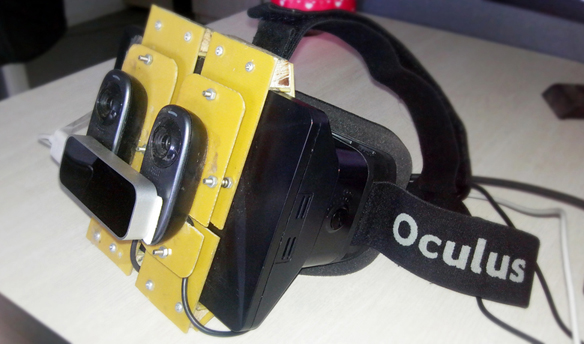
\includegraphics[width=0.6\textwidth]{chap2/ARGlassv1}
  \bicaption[fig:ARGlassesV1.0]{ARGlasses V1.0}{ARGlasses V1.0}{Fig.}{ARGlassesV1.0}
\end{figure}
图\ref{fig:ARGlassesV1.0}为混合现实眼镜的最初设计,由两个USB相机捕获彩色数据,放置在最前方,由Leap Motion捕获手指骨骼,安置在中间,然后通过自制的固定夹板将输入设备固定在Oculus VR上,用户可以通过Oculus VR看到输入设备捕获的现场从而达到视频透视。
在夹板上设有许多旋钮,可以简单调整相机的位置与角度,使两个相机互相间尽量保持一致的相对位置,且达到理想的标定误差。
初代设计的缺陷其一是质量太重,在实验过程中几乎所有参与者都在摘下眼镜后眼睛略感不适并反馈有点沉。
其二则是视野太窄,一个普通摄像头的水平视角在39°,垂直视角在31°,为了达到双目效果横置两个摄像头,于是每个眼睛的水平视角则为31°,与人眼本身接近平角的观察范围相差甚远,观察到的景象会有放大的感觉,让用户失去对深度的正确判断,故而第二个版本主要针对视角进行修改。

\subsubsection{混合现实眼镜广角版}
\begin{figure}[!htp]
  \centering
  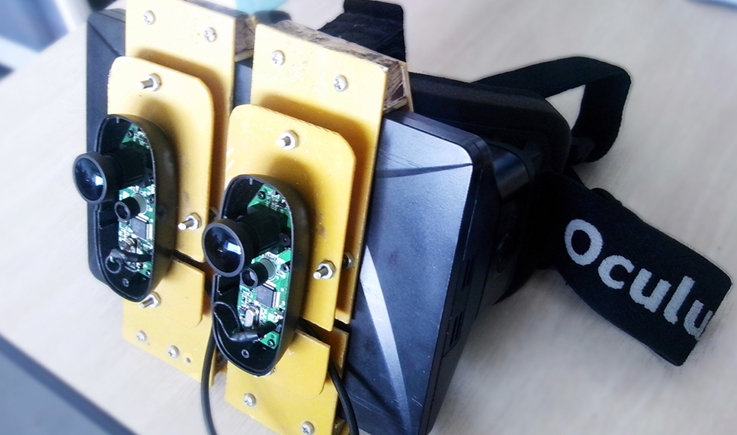
\includegraphics[width=0.6\textwidth]{chap2/ARGlassv2}
  \bicaption[fig:ARGlassesV2.0]{ARGlasses V2.0}{ARGlasses V2.0}{Fig.}{ARGlassesV2.0}
\end{figure}

图\ref{fig:ARGlassesV2.0}主要针对视角进行修改,可以看到原先的USB相机被拆到电路板层级并在摄像头元件前端安置了两个180°广角镜头,安装之后水平视角达到72°,虽然距离人眼的自然视角仍有距离,但比初代版本要宽广一些,并且质量上并没有很大变化。
但初代和广角版共同的缺陷在于双目相机之间的标定,双目标定可以做到对某一深度的物体进行匹配,从而左右眼可以合作观察该深度的物体,但是对于其他深度就会出现标定不合的情况,这是自制双目相机与视频透视融合的缺陷,也是接下来要解决的主要问题。

\begin{figure}[!htp]
  \centering
  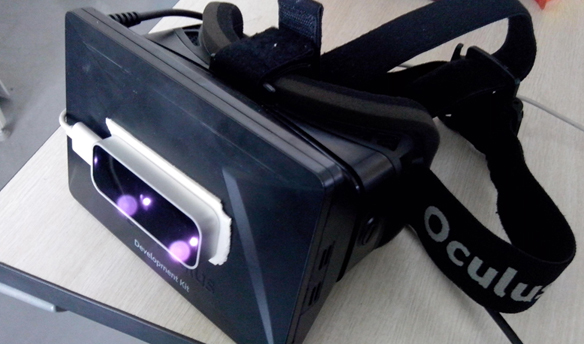
\includegraphics[width=0.6\textwidth]{chap2/ARGlassv3}
  \bicaption[fig:ARGlassesV3.0]{ARGlasses V3.0}{ARGlasses V3.0}{Fig.}{ARGlassesV3.0}
\end{figure}

\subsubsection{混合现实眼镜轻量级}

图\ref{fig:ARGlassesV3.0}则是最新版本,出于轻便性、视野及图像匹配的考虑,本文所设计的系统放弃彩色图像来源,直接使用Leap Motion作为唯一图像输入。
Leap Motion由于本身设备使用多角度的红外摄像头加灰阶Camera采集,可以捕捉到黑白景象,黑白灰阶随深度和热量而变。
其分辨率为640*240,虽然不高但和显示设备Oculus VR的800*600也相去不远。
\begin{table}[!hptb]\renewcommand{\arraystretch}{1.2}
  \centering
  \bicaption[table:arglass]{本文工作所制作的三代混合现实眼镜对比}{本文工作所制作的三代混合现实眼镜对比}{Table}{Comparison among three generations of Mixed Reality Glasses in this work}
  \begin{tabular}{*{4}{L{.32\textwidth}}} \toprule
  %\begin{tabular}{@{}ccc@{}} \toprule
    眼镜名称 & 优点 & 缺点 \\
	\midrule
    混合现实眼镜初代 	& 		1.彩色图像 		& 	\hspace{150pt}1.笨重\hspace{90pt}2.视野狭窄\hspace{90pt}3.存在设备间标定误差\\	
	%&&2.视野狭窄\\
	%&&3.存在设备间的标定误差\\
	%\vspace{1em}
    混合现实眼镜广角版 & 1.彩色图像\hspace{80pt}2.视野有扩大\vspace{1em}& 1.仍显笨重\hspace{90pt}2.存在设备间标定误差\\
	%&2.视野有扩大 &2.存在设备间的标定误差	\\
	%\vspace{1em}
    混合现实眼镜轻量级 & 1.视野符合人眼\hspace{100pt}2.轻巧\hspace{100pt}3.单一输入设备无标定误差& 1.灰色图像 \\
	%&2.轻巧 &\\
	%&3.单一输入设备无标定误差&\\
	\bottomrule
  \end{tabular}
\end{table}
关键其一他的视角到达110°以上,戴上之后和直接视物差距不大,其二由于是将一个完整的场景分割为左右眼两幅图像传递给用户,于是并没有两幅图像间不匹配的困扰,同时由于少了USB相机和固定用的夹板,整个设备一下子轻了很多。
最终三维界面与操控的设计基于混合现实眼镜初代,而三维建模应用的设计基于混合现实眼镜轻量级实现。

\section{本章小结}
本章概要地描述了本文系统的研究方法,然后介绍了本文系统的流程与模块划分,通过本章可以直观明朗地了解到本文系统的输入输出与用例,方便在对其中细节更深的探索前有一个完整的概念。
然后介绍了本文所设计的系统依赖的硬件设备:自制的混合现实眼镜,讲述其构造与发展历程,三代混合现实眼镜的比较可见表\ref{table:arglass}。
本文系统都构建在该设备之上,虽然硬件制作不是本文的重点,但其准确率、精度与轻便性对本文所设计的系统的实验评估都有很大影响,在此处特别介绍下。

%%==================================================
%% chapter03.tex for SJTU Master Thesis
%% Encoding: UTF-8
%%==================================================

\chapter{混合现实眼镜下的三维界面设计}
\label{chap:3DUI}

本章将介绍本文所设计的混合现实眼镜交互系统的第一个部分:三维界面。
三维界面的想法来源于增强现实应用中用户所触及到的三维事物。
大家已经熟悉的桌面应用界面为WIMP系列,二维的界面对应二维的输入,而现在手机、平板上的界面也开始随着设备慢慢地变化,由此本文所设计的系统根据整个操控环境都是三维的前提专门设计了一套三维界面。首先介绍适合增强现实交互界面的设计原则,接着呈现效果,这套三维交互界面将应用在第\ref{chap:interaction}章的交互研究中。

\section{设计原则}

基于\ref{sec:related-cur}节调研的研究现状,本节首先总结出适合增强现实交互界面的设计原则。
该原则主要为避免对识别准确性的影响,减少用户的记忆负担,同时增强交互的用户体验,列举如下:

\label{sec:design-principle}
\begin{enumerate}
\item 不在手上佩戴笨重的设备

由\ref{sec:related-jiaohu}节提到的相关工作可以看到不少精心制作的增强现实设备,然而若是佩戴复杂或者笨重的设备在手上会导致两个问题。
其一,用户体验下降,除了交互之外用户还会被设备的触感,重量等干扰,无法更自如地进行交互;
其二,用户极有可能在使用过程中对设备造成人为影响,比如无意中影响了预设的配置环境,旋转了uTrack\upcite{uTrack}
上的传感器,就会影响输入检测的正确性。
因此从舒适性和正确性角度出发,本文系统的设备将尽量减少手上复杂或笨重的设备佩戴。

\item 保持交互的一致性

试想如果一个增强现实应用中的操控和物理世界有着对应,却用着截然不同的交互手段,则势必会影响用
户在操控时的感受,并且增加记忆的复杂度。所以尽量保留物理世界的交互方式有助于用户尽快适应系统。
同时在物理世界无法做到的功能上,体现增强现实交互的优势,比如用户无法碰触远方的物体因而无法操控,但在增强现实应用环境下就可以实现这一点,
本文工作在对交互一致性的保持上进行改进的设计。

\item 尽可能少的手势设计

这一点同样是出于帮助用户快速适应改进后系统的考虑。
如果一个系统的手势指令太多,用户的记忆复杂度就会增加,可能需要进行一定时间的训练或者每次
都要仔细回顾一番才能再一次适应该系统。
为了让用户迅速学会使用该系统且经久不忘,本文系统最终只设计了三个手势,将在第\ref{chap:interaction}章中详述。

\item 明显的状态切换

在\ref{sec:related-zhuangtai}节中提到通过遮盖两个图案来进行状
态切换的系统\upcite{TrackingBased}。
在实验中,用户经常忘记遮盖指定图案来发送指令,也就是由于状态切换的指令不够明显和
简单,给使用者增加了难度,导致用户的错误指令,
故而系统将设计简单明了的状态切换方式,提升易用性。

\end{enumerate}

根据以上原则,本文设计了手掌召唤式菜单、目标跟踪式菜单和屏幕固定式这三种菜单,具体阐述如下。

%\section{设计结果展示}

\section{手掌召唤式菜单}
\label{sec:palm-based}
\begin{figure}[!htp]
  \centering
  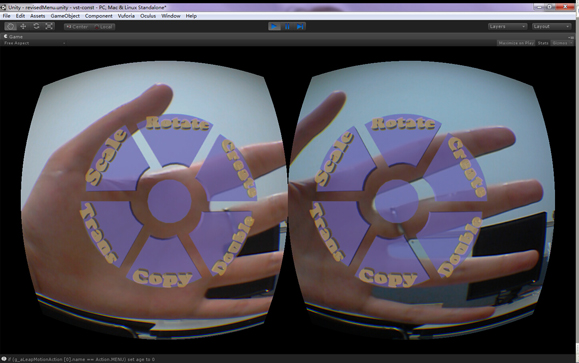
\includegraphics[width=0.8\textwidth]{chap3/palm-basedMenu}
  \bicaption[fig:palm-based]{手掌召唤式菜单}{手掌召唤式菜单}{Fig.}{Palm-based menus}
\end{figure}

手掌召唤式菜单是用户通过手掌手势召唤而
成的菜单,顾名思义位置始终固定在手掌上。为了让菜单和用户
更加融合,本文所设计的系统依据手掌的形状,借鉴调色盘的
概念设计出了该菜单,也是区别于以往直接将二维菜单或者基本图元照搬的一个特点。
用户通过拣选菜单上不同的
指令,然后选中物体对其进行相应的操作,就如同
将调色盘上不同的颜色分配在不同的物体上一样。
如图\ref{fig:palm-based}所示,当摄像头捕获到菜单指令后,在用户手掌正中心出现的就是该菜单,就像是用户手握的一个道具一样。

手掌召唤式菜单含有以下几个选项:创建物体、单手移动物体、单手旋转物体、单手放缩物体、双手操控物体和拷贝物体。
操控类菜单选中后需要指定目标物,可以一个,可以多个。
用户单手操控物体时需要选择不同指令进行不同操作,而用户双手操控物体时,只需要选择双手操控物体的命令即可。
随后系统将根据用户双手间的相对移动,以时间为轴判断用户在进行平移放缩还是旋转。

\section{目标跟踪式菜单}
\begin{figure}[!htp]
  \centering
  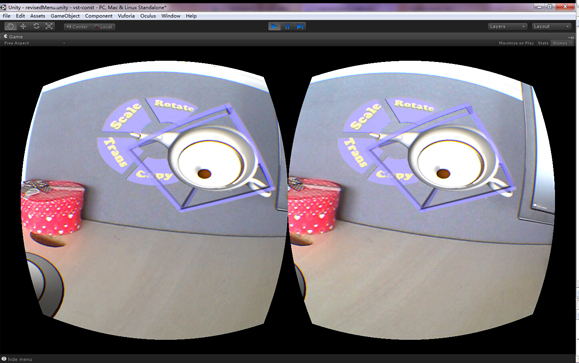
\includegraphics[width=0.8\textwidth]{chap3/object-trackedMenu}
  \bicaption[fig:object-tracked]{目标跟踪式菜单}{目标跟踪式菜单}{Fig.}{object-tracked menus}
\end{figure}

目标跟踪式和手掌召唤式菜单触发方式属于两种类型,后者通过用户的手召唤出来,是基于操作的一种菜单调用;
而前者则是通过选中场景内已经存在的物体,目标跟踪式菜单会出现在该物体周围,随物体的位置变化而变化,选择具体的指令后,该指令就会作用在被选中的物体上,属于基于目标物的一种菜单调用。
如图\ref{fig:object-tracked}所示,召唤出的菜单卡在被选中目标物的一侧。

目标跟踪式菜单有以下几个选项:单手移动物体,单手旋转物体,单手放缩物体,双手操控物体和拷贝物体。和\ref{sec:palm-based}节的功能描述类似。
在操作顺序上由于已经选中物体,于是选完菜单后就可以直接进行操控。

\section{屏幕固定式菜单}
\begin{figure}[!htp]
  \centering
  \subfigure{\label{fig:screen-fixed:1}}\addtocounter{subfigure}{-2}
	\subfigure[Screen-fixed menus sample one]{\subfigure[屏幕固定式菜单示例一]
		{\includegraphics[width=0.4\textwidth]{chap3/screen-fixedMenu1}}}
	\subfigure{\label{fig:screen-fixed:2}}\addtocounter{subfigure}{-2}
	\subfigure[Screen-fixed menus sample two]{\subfigure[屏幕固定式菜单示例二]
		{\includegraphics[width=0.4\textwidth]{chap3/screen-fixedMenu2}}}
  \bicaption[fig:screen-fixed]{屏幕固定式菜单}{屏幕固定式菜单}{Fig.}{Screen-fixed menus}
\end{figure}

屏幕固定式菜单和目标跟踪式菜单的触发方式相同,都属于基于目标物的菜单调用,但选中物体后,屏幕固定式菜单会固定在屏幕正中央,无论选中的物体在哪里,用户如何改变视角,该菜单都会出现在相同的位置,大小和角度都不会变化。
如图\ref{fig:screen-fixed}(a)所示,当选中了茶壶后,茶壶附近出现选中立体框,并在屏幕正中央出现菜单,
而后佩戴ARGlasses的用户向左转头如图\ref{fig:screen-fixed}(b)所示,整个场景变动,茶壶不在视野范围内,但该菜单依然固定在屏幕正中央。

以上三种菜单中,手掌召唤式菜单属于基于操作的菜单类型,选择统一的菜单指令后,可以将指令附着到多个物体上。
而目标跟踪式菜单与屏幕固定式菜单从单个物体出发,偏向个性化操作。
三种菜单在混合现实眼镜下的效果会在第\ref{chap:exp}章详细评估。

\section{三种布局的菜单对照与分析}

\begin{table}[!hpbt]\renewcommand{\arraystretch}{1.1}
  \centering
  \bicaption[table:3dmenu]{本文工作所设计的三种菜单对比}{本文工作所设计的三种菜单对比}{Table}{Comparison among three styles of 3D menus in this work}
\begin{tabular}{*{4}{L{.23\textwidth}}} \toprule
    分析内容 & 手掌召唤式菜单 & 目标跟踪式菜单 & 屏幕固定式菜单 \\
	\midrule
    特点描述 	&
	随手掌召唤而出,位置随手变化 		&
 	由选中物体触发,位置随物体变化 &
	%\vspace{1em}
	\hspace{100pt}由选中物体触发,位置固定在屏幕正中央\\	
	%\vspace{0.5em}
	设计原则一:\hspace{15pt}不在手上佩戴笨重的设备 &
	无任何佩戴物 &
	需佩戴色环选中物体 &
	需佩戴色环选中物体 &\\
%	\vspace{0.8em}
	设计原则二:\hspace{15pt}保持交互的一致性 &
	额外设计手掌触发菜单 &
	选中物体出菜单,与二维菜单习惯一致 &
	选中物体出菜单,与二维菜单习惯一致 &\\
%	\vspace{1em}
	设计原则三:\hspace{15pt}尽可能少的手势设计&
	新增手掌手势&
	选择手势与日常选中手势相似&
	选择手势与日常选中手势相似&\\
%	\vspace{0.3em}
	设计原则四:\hspace{15pt}明显的状态切换&
	通过手掌识别菜单模式&
	通过色环分离控制与选择指令&
	通过色环分离控制与选择指令&
	\bottomrule
  \end{tabular}
\end{table}

由表\ref{table:3dmenu}可见本文设计的三种布局的菜单。手掌召唤式菜单随手掌召唤而出,然后指定物体,是操作先于目标的一种思考方式,
目标跟踪式菜单指定物体然后显示,和屏幕固定式菜单相同,是目标先于操作的一种思考方式。
而这二者的区别在于菜单的位置,前者随目标物移动,而后者固定在屏幕中央。
前者的设计思路将菜单作为目标物的一种属性,将菜单镶嵌在目标物周围;
后者从更直观的显示角度出发。
在设计原则的应用上,三者都尽量减少了额外的佩戴物,即便是色环也是轻量级的物体;
手掌召唤式菜单额外增加了手掌召唤菜单的交互,但并没有和现实生活中的交互产生矛盾,对用户产生的记忆压力也不大,另两者没有新增交互和手势设计;
最后手掌手势和色环成功分离了自己的状态和其他状态,做到了明显的状态切换这一原则。

\section{本章小结}
本章主要介绍了本文所设计的系统使用的三维界面。
首先通过对相关工作的理解提出了设计原则,设计原则应用于三维界面设计。
然后列举了设计的三种菜单。
手掌召唤式菜单以操作为重点,先选菜单再选目标物,并且手掌召唤式菜单卡位于掌心,将用户的手变成了一个增强现实界面。
目标跟踪式菜单和屏幕固定式菜单均以目标物为重点,先选择想要操作的物体,然后再选择想要实行的功能。
并且采用了两种风格的布局,目标跟踪式菜单会随目标物而移动,屏幕固定式菜单则始终固定在屏幕正中央,无论用户看向何方都能看到嵌在屏幕中央的菜单,便于选择。
除此之外介绍了本文系统设计的几个菜单,分别是创建、单手操控菜单组、双手操控和拷贝物体。
对菜单进一步的评估将在第\ref{chap:exp}章展开。
\include{body/conclusion} %% 全文总结


%%%%%%%%%%%%%%%%%%%%%%%%%%%%%% 
%% 附录(章节编号重新计算,使用字母进行编号)
%%%%%%%%%%%%%%%%%%%%%%%%%%%%%% 
\appendix

% 附录中编号形式是"A-1"的样子
\renewcommand\theequation{\Alph{chapter}--\arabic{equation}}
\renewcommand\thefigure{\Alph{chapter}--\arabic{figure}}
\renewcommand\thetable{\Alph{chapter}--\arabic{table}}

%%==================================================
%% app1.tex for SJTU Master Thesis
%% based on CASthesis
%% modified by wei.jianwen@gmail.com
%% version: 0.3a
%% Encoding: UTF-8
%% last update: Dec 5th, 2010
%%==================================================

\chapter{模板更新记录}
\label{chap:updatelog}

\textbf{2013年5月26日} v0.5.3发布,更正subsubsection格式错误,这个错误导致如"1.1 小结"这样的标题没有被正确加粗。

\textbf{2012年12月27日} v0.5.2发布,更正拼写错误:从``个人建立''更正为``个人简历''。在diss.tex加入ack.tex,更名后忘了引用。

\textbf{2012年12月21日} v0.5.1发布,在 \LaTeX 命令和中文字符之间留了空格,在Makefile中增加release功能。

\textbf{2012年12月5日} v0.5发布,修改说明文件的措辞,更正Makefile文件,使用metalog宏包替换xltxtra宏包,使用mathtools宏包替换amsmath宏包,移除了所有CJKtilde(\verb+~+)符号。

\textbf{2012年5月30日} v0.4发布,包含交大学士、硕士、博士学位论文模板。模板在\href{https://github.com/weijianwen/sjtu-thesis-template-latex}{github}上管理和更新。

\textbf{2010年12月5日} v0.3a发布,移植到 \XeTeX/\LaTeX 上。

\textbf{2009年12月25日} v0.2a发布,模板由CASthesis改名为sjtumaster。在diss.tex中可以方便地改变正文字号、切换但双面打印。增加了不编号的一章“全文总结”。
添加了可伸缩符号(等号、箭头)的例子,增加了长标题换行的例子。

\textbf{2009年11月20日} v0.1c发布,增加了Linux下使用ctex宏包的注意事项、.bib条目的规范要求,
修正了ctexbook与listings共同使用时的断页错误。

\textbf{2009年11月13日} v0.1b发布,完善了模板使用说明,增加了定理环境、并列子图、三线表格的例子。

\textbf{2009年11月12日} 上海交通大学硕士学位论文 \LaTeX 模板发布,版本0.1a。

 % 更新记录
%% app2.tex for SJTU Master Thesis
%% based on CASthesis
%% modified by wei.jianwen@gmail.com
%% version: 0.3a
%% Encoding: UTF-8
%% last update: Dec 5th, 2010
%%==================================================

\chapter{Maxwell Equations}

选择二维情况,有如下的偏振矢量
\begin{subequations}
  \begin{eqnarray}
    {\bf E}&=&E_z(r,\theta)\hat{\bf z} \\
    {\bf H}&=&H_r(r,\theta))\hat{ \bf r}+H_\theta(r,\theta)\hat{\bm
      \theta}
  \end{eqnarray}
\end{subequations}
对上式求旋度
\begin{subequations}
  \begin{eqnarray}
    \nabla\times{\bf E}&=&\frac{1}{r}\frac{\partial E_z}{\partial\theta}{\hat{\bf r}}-\frac{\partial E_z}{\partial r}{\hat{\bm\theta}}\\
    \nabla\times{\bf H}&=&\left[\frac{1}{r}\frac{\partial}{\partial
        r}(rH_\theta)-\frac{1}{r}\frac{\partial
        H_r}{\partial\theta}\right]{\hat{\bf z}}
  \end{eqnarray}
\end{subequations}
因为在柱坐标系下,$\overline{\overline\mu}$是对角的,所以Maxwell方程组中电场$\bf
E$的旋度
\begin{subequations}
  \begin{eqnarray}
    &&\nabla\times{\bf E}=\mathbf{i}\omega{\bf B} \\
    &&\frac{1}{r}\frac{\partial E_z}{\partial\theta}{\hat{\bf
        r}}-\frac{\partial E_z}{\partial
      r}{\hat{\bm\theta}}=\mathbf{i}\omega\mu_rH_r{\hat{\bf r}}+\mathbf{i}\omega\mu_\theta
    H_\theta{\hat{\bm\theta}}
  \end{eqnarray}
\end{subequations}
所以$\bf H$的各个分量可以写为:
\begin{subequations}
  \begin{eqnarray}
    H_r=\frac{1}{\mathbf{i}\omega\mu_r}\frac{1}{r}\frac{\partial
      E_z}{\partial\theta } \\
    H_\theta=-\frac{1}{\mathbf{i}\omega\mu_\theta}\frac{\partial E_z}{\partial r}
  \end{eqnarray}
\end{subequations}
同样地,在柱坐标系下,$\overline{\overline\epsilon}$是对角的,所以Maxwell方程组中磁场$\bf
H$的旋度
\begin{subequations}
  \begin{eqnarray}
    &&\nabla\times{\bf H}=-\mathbf{i}\omega{\bf D}\\
    &&\left[\frac{1}{r}\frac{\partial}{\partial
        r}(rH_\theta)-\frac{1}{r}\frac{\partial
        H_r}{\partial\theta}\right]{\hat{\bf
        z}}=-\mathbf{i}\omega{\overline{\overline\epsilon}}{\bf
      E}=-\mathbf{i}\omega\epsilon_zE_z{\hat{\bf z}} \\
    &&\frac{1}{r}\frac{\partial}{\partial
      r}(rH_\theta)-\frac{1}{r}\frac{\partial
      H_r}{\partial\theta}=-\mathbf{i}\omega\epsilon_zE_z
  \end{eqnarray}
\end{subequations}
由此我们可以得到关于$E_z$的波函数方程:
\begin{eqnarray}
  \frac{1}{\mu_\theta\epsilon_z}\frac{1}{r}\frac{\partial}{\partial r}
  \left(r\frac{\partial E_z}{\partial r}\right)+
  \frac{1}{\mu_r\epsilon_z}\frac{1}{r^2}\frac{\partial^2E_z}{\partial\theta^2}
  +\omega^2 E_z=0
\end{eqnarray}
 % 麦克斯韦方程
% \include{body/app3}


%%%%%%%%%%%%%%%%%%%%%%%%%%%%%% 
%% 文后(无章节编号)
%%%%%%%%%%%%%%%%%%%%%%%%%%%%%% 
\backmatter

% 参考文献
% 使用 BibTeX
% 包含参考文献文件.bib
\bibliography{reference/chap1,reference/chap2}

%% 个人简历(硕士学位论文没有个人简历要求)
% %%==================================================
%% resume.tex for SJTU Master Thesis
%% based on CASthesis
%% modified by wei.jianwen@gmail.com
%% version: 0.3a
%% Encoding: UTF-8
%% last update: Dec 5th, 2010
%%==================================================

\begin{resume}

\begin{resumesection}{基本情况}
xxx,男,上海人,1985 年~12 月出生,未婚,
上海交通大学物理系在读博士研究生。
\end{resumesection}

\begin{resumelist}{教育状况}
XXXX 年~9 月至~XXXX 年~7 月,上海交通大学, 本科,专业:XXXX

XXXX 年~9 月至~XXXX 年~7 月,上海交通大学, 硕士研究生,专业:XXXX

XXXX 年~9 月至~XXXX 年~7 月,上海交通大学,
博士研究生(提前攻读博士),专业:XXXX
\end{resumelist}

\begin{resumelist}{工作经历}
无。
\end{resumelist}

\begin{resumelist}{研究兴趣}
XXXXXXX。
\end{resumelist}

\begin{resumelist}{联系方式}
通讯地址:上海市闵行区东川路800号,上海交通大学物理系

邮编:200240

E-mail: abcde@sjtu.edu.cn
\end{resumelist}

\end{resume}


% 致谢
%%==================================================
%% thanks.tex for SJTU Master Thesis
%% based on CASthesis
%% modified by wei.jianwen@gmail.com
%% version: 0.3a
%% Encoding: UTF-8
%% last update: Dec 5th, 2010
%%==================================================

\begin{thanks}

  感谢杨旭波教授的指导!
  
  感谢数字艺术实验室全体,前前后后在这里几乎四年,从送走敬仰的前辈到自己即将离开,非常高兴能和大家相遇。
  
  感谢所有被我压榨过来艰难苦恨做实验的同学,请随时随地来领糖!
  
  感谢何国胜同志亲自操刀帮我做的ARGlasses初代版的夹板,惊为天人。
  
  如今我们要各奔前程,希望大家求仁得仁,实验室A类不断,终有所得。

\end{thanks}


% 发表文章目录
%%==================================================
%% pub.tex for SJTU Master Thesis
%% based on CASthesis
%% modified by wei.jianwen@gmail.com
%% version: 0.3a
%% Encoding: UTF-8
%% last update: Dec 5th, 2010
%%==================================================

\begin{publications}{99}

    \item\textsc{He Zhenyi, Yang Xubo}. {Object creation based on free virtual grid with ARGlass}[C]//SIGGRAPH Asia 2014 Posters. ACM, 2014: 41.

    \item\textsc{He Zhenyi, Yang Xubo}. {Hand-based interaction for object manipulation with augmented reality glasses}[C]//Proceedings of the 13th ACM SIGGRAPH International Conference on Virtual-Reality Continuum and its Applications in Industry. ACM, 2014: 227-230.
    
\end{publications}


% 参与项目列表
%%==================================================
%% projects.tex for SJTU Master Thesis
%% based on CASthesis
%% modified by wei.jianwen@gmail.com
%% version: 0.3a
%% Encoding: UTF-8
%% last update: Dec 5th, 2010
%%==================================================

\begin{projects}{99}

    \item 973项目“XXX”
    \item 自然基金项目“XXX”
    \item 国防项目“XXX”
    
\end{projects}


\end{document}
